\ifdefined\included
\else
\setcounter{chapter}{4} %% Numéro du chapitre précédent ;)
\dominitoc
\faketableofcontents
\fi

\chapter{Ontology-based Referring Expression Generation}
\chaptermark{Ontology-based REG}
\minitoc

The contribution presented in this chapter is excerpted from our work, published in the proceedings of the RO-MAN 2020 conference~\cite{buisan_2020_efficient}. In this manuscript, the contribution is more detailed and discussed. The presented work has been achieved in collaboration with Guilhem Buisan, with an equal contribution. Several algorithms have been developed by both of us, giving, as a result, the one presented in this chapter, merging the best of our trials. My focus was mainly on how to fully take advantage of the ontology as a knowledge base and on algorithmic optimisations to make our method the most efficient in the current literature.

\section{Introduction}

Referring to an entity is one of the most common task that we perform every day. "Can you bring me my mug? It is the black one next to the sink". "I don't remember the name of the man with the red shirt and the glasses". "I lost my keys, they are on a keychain with a soft toy in the shape of a unicorn". Such kind of communication, precise and efficient, are a key apect for the success of a collaborative tasks. Nevertheless, in complex environment with a wide variety of objects, places, or people, referring a specific entity can become a real challenge for robotic application. The robot has to take into account the context of the upper task, the diversity of facts that can be extracted from the situation and which depend on available perception modalities, and the available common ground between the robot and its partner. 

\begin{figure}[h!]
\centering
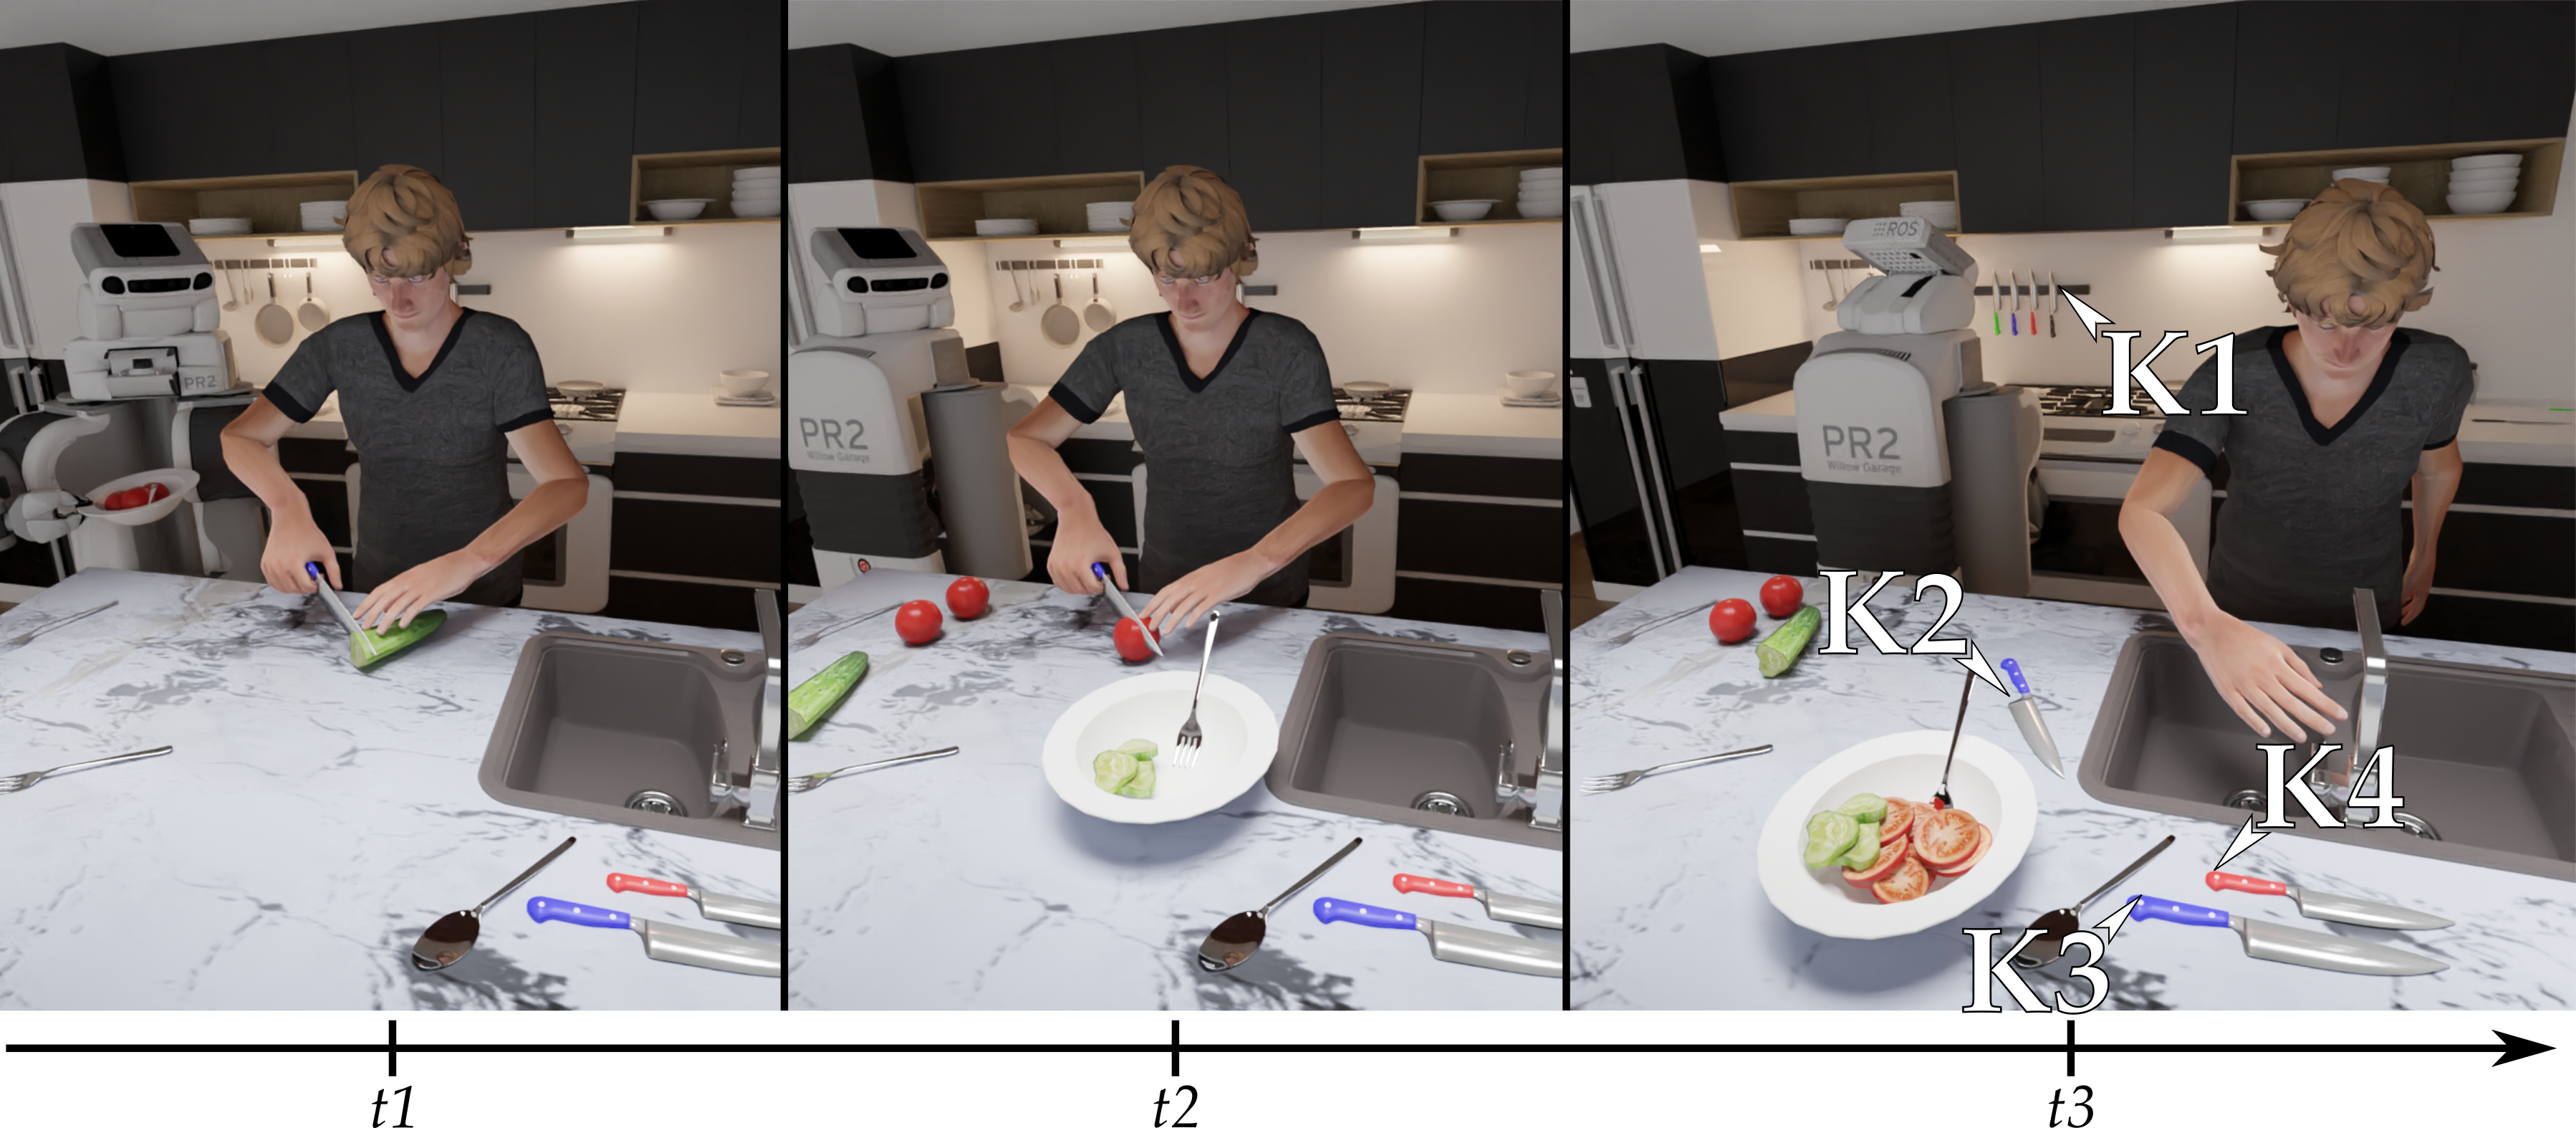
\includegraphics[scale=0.16]{figures/chapter4/intro.png}
\caption{\label{fig:chap4_intro} Six situations view from the hearer perspective, with the robot placed on the other side of the table. Referring to the same pen involves different mechanisms to raise the ambiguity, in each situation. The sentence above each situation is a possible referring expression to designate the said pen without ambiguity. }
\end{figure}

Consider the situation where you are around a table with your collaborative robot and the robot needs a pen. The simple statement \textit{"Give me the pen"} can result in several situations of different complexities. In the case where there is only one pen (Fig.\ref{fig:chap4_intro}a), the referring it is obvious. Now consider two pens on the table. If one is reachable by you (the human) and the other is not (Fig.\ref{fig:chap4_intro}b), reachability can be used to refer to the pen. If both pens are not reachable but one is visible to you and the other is not (Fig.\ref{fig:chap4_intro}c where a pen is hidden under the box), visibility through perspective-taking could be used to determine that the other pen does not lead to ambiguity. Now both pens are visible and reachable, but one is blue and the other is red (Fig.\ref{fig:chap4_intro}d). The addition of the color of the pen solves the ambiguity. If both pens have the same color but one is in a pencil box (Fig.\ref{fig:chap4_intro}e), the relation to the pencil box resolves the ambiguity. If unfortunately, both are in a pencil box but one is green and the other orange (Fig.\ref{fig:chap4_intro}f), the relation to the pencil box and the color of the latter resolves the ambiguity. We could continue like this for a long time, considering that one is at your left and one at your right, that there is no pen on the table but there is one on a shelf and so on.

Until now, we considered that the robot knows the concepts of pen and pencil box as well as their names in natural language to speak about them. However, imagine yourself travelling in another country and having to speak english\footnote{I apologize to the native English speakers who will not take full advantage of this example.}, you can sometimes miss some words and thus use more generic a one instead. However, by doing so some new ambiguity can be raised because this generic word also refers to other entities. It is the same for our robot if it has to speak French and does not know the translation of the pencil box concept. It will have to resort to a more generic term, such as "container" that can also refer to a box beside.

In addition to the concepts names, the robot must pay attention to the relationships it uses. The exact weight or length of an object wouldn't be useful as a human can not easily evaluate them. On the contrary, the color of the object seems to be a suitable property to use, unless the robot partner is color blind. This means that the robot has to use relations that it estimates to be known and observable by its partner. Such can be done considering the theory of mind and performing the generating the entity reference on the estimation by the robot of the knowledge base of the human partner.

This task to refer to a precise entity among others is commonly called the \textbf{Referring Expression Generation} (REG) task. It is often decomposed into two sub-tasks: the \textbf{content determination} and the \textbf{linguistic realisation}~\cite{krahmer_2012_computational}. The content determination aims at determining the relations to be used to refer to an entity while the linguistic realisation aims at choosing the words to be used to communicate the content. The contribution of this chapter is focused on content determination but we can not consider these two sub-tasks entirely independent. As explained earlier, if the robot does not know some concept names in natural language, the linguistic realisation will fail in the case the content determination select them or the linguistic realisation will choose a more general word that does not correspond to the determined content. We could imagine a dedicated knowledge base for the REG with only concepts usable in natural language, but such a solution is not suitable if we want a unique knowledge base for all the robotic system. Moreover, it could be hard to maintain this dedicated knowledge base during the interaction, in addition to others. 

The main contribution presented in this chapter is an \textbf{ontology-based and domain-independent algorithm for the generation of referring expressions}. It uses customizable cost function estimating the cognitive load required for a human to interpret the RE to produce \textbf{the optimal set of verbalizable assertions} that allows to refer unambiguously a given entity.

First, we review the literature concerning the REG problem and discuss the issues we aim to tackle. Then, we refine the definition of the problem to manage it at a search problem in a second part. We then compare our algorithm with two states of the art algorithms to assess its solutions and its performance. We end this chapter with integration on a real robotic system with some detail on the used perception system and the verbalization method.

\section{Related work}

Referring Expression Generation is a today classic task in Natural Language Generation \cite{gatt_2018_survey} that has been studied for decades. It has been defined by Reiter as the concern of "how we produce a description of an entity that enables the hearer to identify that entity in a given context"~\cite{reiter_2000_building}. Over time, the criteria for a good Referring Expression (RE) have been refined but still take their roots from the Grice's maxims~\cite{grice_1975_logic}. The maxim of \textit{manner} requires the communication to be unambiguous. It is also the referential success for the target entity to be unambiguously identified by the RE hearer. The maxim of \textit{relation} requires the communication to be relevant regarding the current context both the context of the task to achieve and the current world state. If you are asking someone to give you an object that is in the room where you are, you can reasonably assume that the objects in the rest of the house are not ambiguous with the one you are requesting. The maxim of \textit{quality} seems to be evident and requires the communication to be true. If you are asking a bootle and you do not know if it is full or not, you should not use this information to refer to the bottle. Finally, the maxim of \textit{quantity} requires the communication to be as informative as required but not more informative than required. In simple words, to be brief. In the context of REG, the hearer must understand quickly want you are talking about. Moreover, giving unnecessary information could lead to false implications. Saying "give me the red pen" could imply that at least one other non-red pen exists and such warn the hearer to not do the mistake to take the wrong one. If no other pen exists regarding the current context, the sentence "give me the pen" is thus sufficient.

Dale and Reiter are considered as being the pioneers of the Referring Expression Generation and have proposed over years three main algorithms solving it. Two first two fundamental approaches are the Depth First Search (DFS)~\cite{dale_1989_cooking} and the Full Brevity~\cite{dale_1992_generating}. While the first algorithm does not always find an optimal solution in terms of the number of relations used, the second does it at the cost of an exhaustive search. The most notable advance was thus the Incremental Algorithm (IA) first presented in~\cite{reiter_1992_fast} then refine in~\cite{dale_1995_computational}. With this algorithm, the notion of preference over features has been highlighted. This notion aims at representing the fact that some features are easier to understand than others. For example, the color or the shape of an object is easier the understand than spatial relations. However, the major limitation of the presented algorithms is the used knowledge representation. Because they used a set of attribute-value pairs for each entity, the solutions can only be composed of entity attributes and cannot use relations between entities. To be more precise, the algorithms can give the fact the referred entity is on a table but cannot discriminate the said table among others.

With the introduction of a new representation in the form of a labeled directed multi-graph (also known as the REG graph), Krahmer et al. solved the issue of the reference to other entities~\cite{krahmer_2003_graph}. The related Graph-Based Algorithm (GBA) REG is able to manage relations between entities and, as Dale and Reiter, consider a preference over features. This preference, called Preference Ordering (PO), is represented by a cost assigned to each edge of the graph. The GBA algorithm uses a branch\&bound algorithm which allows finding the optimal RE. On this new basis, extensions have been developed or at least discussed. Regarding the thin link with Description Logic, Krahmer raised the problem of the hierarchy of entity types in~\cite{krahmer_2012_computational}. On its side, Li et al. have proposed an optimized version of the GBA~\cite{li_2017_automatically} GBA allowing an efficiency gain close to 56\%. However, the used task only involved cubes, meaning that their algorithm does not have to take into account the entities' types, which were just added as a post-process. A last interesting GBA is the Longest First (LF) algorithm presented in~\cite{viethen_2013_graphs}. However, more than not respecting the maxim of quantity, its exhaustive search entails poor performance when used on larger realistic knowledge bases.

Learning-based approaches have of course been proposed. The belief network-based method presented in~\cite{yamakata_2004_belief} can only work with objects' attributes. Moreover, the authors indicate that a specific belief network should be constructed and therefore trained for each attribute. Such limitation reduces the genericity of the method. With a log-linear model trained from a corpus of the probability distribution of REs~\cite{fitzgerald_2013_learning}, Fitzgerald et al. face the same problem. Nevertheless, by working on belief bases, Yamakata has highlighted the importance to run the algorithm on the human partner's estimated belief base. It ensures the robot generates a referring solution compatible with concepts estimated to be known by the human.

All the algorithms presented here before are highly dependent on the task to perform. Where learning approaches are dependent on their training corpus, the other relies on knowledge bases integrating only relations usable in the context of the task. Williams et al. proposed a hybrid approach between domain-dependent and domain-independent with a distributed Incremental Algorithm (DIST-PIA)~\cite{williams_2017_referring}. The idea besides this algorithm is to make the core Incremental Algorithm independent of the knowledge representation by making it querying domain-dependent consultants~\cite{williams_2016_framework}. A consultant is an interface of a knowledge base and each knowledge base of the distributed architecture owns one. Each consultant is thus dedicated to a specific set of properties and can be query regarding these properties. To get relations about the location of entities, the Incremental Algorithm can thus query the consultant associated with the knowledge base of locations. While this solution is interesting for distributed architectures, we can ask ourselves about the domain-independence of the core Incremental Algorithm. Indeed, the ordering of the consultants to query in the algorithm can have an impact on the found solution. However, it is worth mentioning that this method has been successfully integrated into a robotic architecture~\cite{williams_2019_dempster}.

At the date, the closest work to the one presented in this chapter is introduced in~\cite{ros_2010_which}. This method uses ontology as a knowledge base. As explained earlier, such knowledge representation is suitable for domain-independent applications. However, here again, the used algorithm takes as a hypothesis that only relations useful for the REG task are present in it. Moreover, in the same way as the IA-based algorithm, their method only supports entities' attributes and not relations between entities. This method has still been integrated into a robotic system that can take advantage of perspective-taking to construct an estimated knowledge base of the human partner to give pertinent RE~\cite{lemaignan_2011_grounding}.

Even if all the presented algorithms rely on different kinds of knowledge representation and have non-equivalent abilities, they all consider a perfect linguistic realisation~\cite{krahmer_2012_computational}. We mean here that they all consider that any concept of their knowledge bases has a word in natural language and can thus be verbalize. Wanting to run on the same knowledge base as the other component of the robotic architecture, we do not want to make this assumption. Even if our contribution is focused on content determination, we aim with this contribution to make a first step in the linguistic realisation by not considering these to sub-task as being independent of one the other. We thus assume that not all the concepts in the knowledge base can be used in natural language.

To give a better overview of the progress in the REG field, the most representative contributions presented above are summarized in Table.~\ref{tab:reg_ref_sumup}. The contributions are organized chronologically and around six major features that we have mentioned throughout this section. These desired features are:
\begin{itemize}
	\item \textbf{Domain independent}: The knowledge base used by the REG must be able to be used by other components of a robotic architecture. The REG algorithm must not consider that all the knowledge represented can be used for this task.
	\item \textbf{Representation type}: The used knowledge representation must be able to be updated all along an interaction to deal with the dynamic of robotic applications.
	\item \textbf{Use of types}: The type of an entity is the minimal information to use to refer to an entity. Without type, linguistic realisation can not be done.
	\item \textbf{Preference ordering (PO)}: Some properties are easier to understand than others. Ordering the properties according to this preference allows finding efficient referring expressions.
	\item \textbf{Referring to other entities}: Entities attributes are not sufficient to find referring expressions in realistic situations. Being able to refer to an entity by referring to another one is thus mandatory.
	\item \textbf{Natural language}: Considering the linguistic realisation during the content generation could prevent the appearance of ambiguity at the linguistic realisation or even the incapacity to perform it.
\end{itemize}

\begin{table}[!h]
\centering
\caption{Summary of the most representative contributions in the REG field regarding the six major features of the problem. The contributions are listed in chronological order to give a better overview of progress in the field.}
\label{tab:reg_ref_sumup}
\begin{tabular}{lcccccc}
\hline
\multicolumn{1}{|c|}{Contributions} & \multicolumn{1}{c|}{\begin{tabular}[c]{@{}c@{}}Domain\\ inde-\\ pendent\end{tabular}} & \multicolumn{1}{c|}{\begin{tabular}[c]{@{}c@{}}Rep.\\ Type\end{tabular}} & \multicolumn{1}{c|}{\begin{tabular}[c]{@{}c@{}}Use of\\ types\end{tabular}} & \multicolumn{1}{c|}{PO}  & \multicolumn{1}{c|}{\begin{tabular}[c]{@{}c@{}}Referring\\ to other\\ entities\end{tabular}} & \multicolumn{1}{c|}{\begin{tabular}[c]{@{}c@{}}Natural\\ language\end{tabular}} \\ [0.5ex] \hline \hline
\cite{dale_1989_cooking}            & \cellcolor{red!25} No                                                                 & \begin{tabular}[c]{@{}c@{}}Knowledge\\ base entity\end{tabular}          & \cellcolor{red!25} No                                                       & \cellcolor{red!25} No    & \cellcolor{red!25} No                                                                        & \cellcolor{red!25} No                                                           \\
\cite{dale_1992_generating}         & \cellcolor{red!25} No                                                                 & -                                                                        & -                                                                           & \cellcolor{red!25} No    & \cellcolor{red!25} No                                                                        & \cellcolor{red!25} No                                                           \\
\cite{reiter_1992_fast}             & \cellcolor{red!25} No                                                                 & \begin{tabular}[c]{@{}c@{}}attribute-\\ value pairs\end{tabular}         & \cellcolor{green!25} Yes                                                    & \cellcolor{green!25} Yes & \cellcolor{red!25} No                                                                        & \cellcolor{red!25} No                                                           \\
\cite{krahmer_2003_graph}           & \cellcolor{red!25} No                                                                 & REG graph                                                                & \cellcolor{red!25} No                                                       & \cellcolor{green!25} Yes & \cellcolor{green!25} Yes                                                                     & \cellcolor{red!25} No                                                           \\
\cite{yamakata_2004_belief}         & \cellcolor{red!25} No                                                                 & \begin{tabular}[c]{@{}c@{}}Belief\\ Network\end{tabular}                 & \cellcolor{red!25} No                                                       & \cellcolor{green!25} Yes & \cellcolor{red!25} No                                                                        & \cellcolor{red!25} No                                                           \\
\cite{ros_2010_which}               & \cellcolor{orange!25} Yes                                                             & Ontology                                                                 & \cellcolor{red!25} No                                                       & \cellcolor{green!25} Yes & \cellcolor{red!25} No                                                                        & \cellcolor{red!25} No                                                           \\
\cite{viethen_2013_graphs}          & \cellcolor{red!25} No                                                                 & REG graph                                                                & \cellcolor{red!25} No                                                       & \cellcolor{green!25} Yes & \cellcolor{green!25} Yes                                                                     & \cellcolor{red!25} No                                                           \\
\cite{williams_2017_referring}      & \cellcolor{orange!25} Yes                                                             & \begin{tabular}[c]{@{}c@{}}Distributed\\ KBs\end{tabular}                & \cellcolor{red!25} No                                                       & \cellcolor{green!25} Yes & \cellcolor{red!25} No                                                                        & \cellcolor{red!25} No                                                           \\
\cite{buisan_2020_efficient}        & \cellcolor{green!25} Yes                                                              & Ontology                                                                 & \cellcolor{green!25} Yes                                                    & \cellcolor{green!25} Yes & \cellcolor{green!25} Yes                                                                     & \cellcolor{green!25} Yes                                                       
\end{tabular}
\end{table}

The literature presented here before is focused on Referring Expression Generation in its nominal form. Some researches have however addressed side problems that we do not aim to tackle. Not entering much in the details, we mention them to give a more global picture of the field. The use of spatial relations is not trivial as these relations can differ for certain entities taking the RE emitter's or receiver's point of view while for other entities, having a clear orientation system (e.g. a car), the relations remain unchanged~\cite{kelleher_2006_incremental, dos_2015_generating}. Spatial relations can also be expressed not only based on a single entity but also according to a set of entity~\cite{fang_2013_towards}. While a RE is often considered as being a single sentence referring to an entity without ambiguity, some see it as a more collaborative task where the RE is provided step by step, allowing to catch acknowledgement and to refine it according to the receiver comprehension~\cite{fang_2014_collaborative, wallbridge_2019_generating}. Finally, some research tries to integrate REG in a more global interaction where several agents refer to entities. The robot thus tries to reuse properties previously used by the partner ensuring that these properties are known~\cite{williams_2020_toward}. Limitations about this work will be discussed later in this thesis.

\section{Define the REG problem}

In this section, we present the ontology of example that we use all along with this chapter. We then discuss how the up-task in which a REG could be performed can restrict the search among the entire knowledge base. Finally, we formally define the expected form for a solution to a REG problem and the constraints it must respect.


\subsection{The knowledge representation}

As presented earlier in this thesis, ontology is a way to represente knowledge that is now largely used in many field becasue it allows a standardization of the representation easy extension of an extisting knowledge base, and the use of inference engine to enrich the the knowledge base. For these reasons, we choose to use a knowledge base in the form of an ontology as input of our algorithm for the REG problem. Moreover, we saw that number of recent REG algorithm have trend to use graph representations as it allows to refer to an entity through relations to other entities. Because an ontology can be see as a more complexe and mor expressive graph, this representation seems to be adequate to use for the REG problem. 

\begin{figure}[h!]
\centering
\includegraphics[scale=0.2]{figures/chapter4/pens.png}
\caption{\label{fig:chap4_kb} A situation view from the hearer perspective, with the robot placed on the other side of the table. Three pens and two cups are on a table. The two blue pens are each in one cup. }
\end{figure}

In this chapter, we take as an example the situation represented in Figure~\ref{fig:chap4_kb}. The situation is assumed to be perceived by the robot and represented in its semantic knowledge base. This knowledge base as an ontology is of the form $\kbs^R = \langle \Abox^R, \Tbox^R, \Rbox^R \rangle$. $\Abox$, $\Tbox$ like presented in Section~\ref{sec:kb_formalism}. The estimated knowledge base of the human partner $\kbs^H$ is here assumed to be the same as that of the robot in the way that $\kbs^R \equiv \kbs^H \equiv \kbs$.

The Tbox used to describe the situation of example is represented in Figure~\ref{fig:chap4_kb_Tbox}. The class IkeaLisabo represent a precise model of tables and does not have any label. The class Pen is specified through two classes the ClickingPen and the TurningPen. These two classes aim at representing the pens you need to click on top to get the tip of the pen out and the pens you need to turn to get the tip of the pen out. These classes do not have any label to directly speak about them. They are such used for the robot to know how to use them. For sure a more precise ontology could be drawn but we try to keep it simple for the purpose of this chapter.

\begin{figure}[h!]
\centering
\includegraphics[scale=0.4]{figures/chapter4/pens_Tbox.png}
\caption{\label{fig:chap4_kb_Tbox} Representation of the Tbox (classes hierarchy) used to describe the situation of the Figure~\ref{fig:chap4_kb}. }
\end{figure}

The Abox used to describe the situation is represented in Figure~\ref{fig:chap4_kb_Abox}. The two cups C\_1 and C\_2 are on the table T\_1. The two pens P\_1 and P\_2 are respectivly in the cups C\_1 and C\_2 while P\_3 is directly on the table. The pen P\_4 is another pen, not on the table. Other objects could be represented as the robot and the human could know other object being in the room. the pen P\_1 is the only pen for which the agent has to click to get the tip of the pen out.

\begin{figure}[h!]
\centering
\includegraphics[scale=0.38]{figures/chapter4/pens_Abox.png}
\caption{\label{fig:chap4_kb_Abox} Representation of the Abox (relation graph) used to describe the situation of the Figure~\ref{fig:chap4_kb}. }
\end{figure}

The Rbox is not represented but the properties composing it are the ones used in the Abox. In addition with define the properties \textit{hasIn} being the inverse of \textit{isIn} and \textit{isUnder} being the inverse of \textit{isOn} ($\{(isIn,\ hasIn), (isOn,\ isUnder)\} \subset \invset$). Moreover, the property \textit{isOn} inherits of the upper property \textit{isAbove} ($\{(isOn,\ isABove), (isUnder,\ isBelow)\} \subset \inclset$). While the first state a direct contact between two entities, the other does not. Finally, we declare the chain axiom: $isIn \bullet isOn \Rightarrow isABove$. This axiom allows to reason on the ontology and declare that if an first entity is in a second one and that this second is on a third one, the first entity is above the third. Taking our example, because P\_1 is in C\_1 that is on T\_1, the pen P\_1 is above the table T\_1.


\subsection{Contextualization and restriction for situated REG}

The human (named Tony) and the robot are involved in a shared task around a table. During the task, the robot needs a blue pen to write. However, It can not take one by itself as the blue pens are on cups. Moreover, with its huge gripper, it can not use the kind of pens where you have to click. Our robot thus precisely need the pen P\_2 of our example and has to ask it to its human partner\footnote{Some could tell that if it is not the first time that our robot and this human collaborate, the human could be aware of the robot capability. In this case, the robot would just have to ask for a blue pen and the task would be over. We thus consider that our robot never had interacted with this particular human. For sure it could explain its capability but the purpose is not there.}.

The robot is thus aiming to unambiguously designate an entity $\goalindiv \in \indivset$ through its attributes and relations to other entities. However, as explained, the REG is meant to be used in the context of an upper task that has to be took into account. In our exampe, the collaborative task concerns object on the table so that the other entities in the room are clearly out of context. Asking for a pen, P\_4 will not lead to any ambiguous situation as it is not on the table around which the interaction is performed. To represent this restiction, we provide the problem a \textbf{context} $Ctx = (\relationset_{ctx}, \inheritset_{ctx})$. It is a set of relation and direct types that are implicit to the current communication with regard to the task. This context is used to find a reference to $\goalindiv$, but has not to be included in the generated RE. For our example the context could be $Ctx = (\{ (\goalindiv,\ isOn,\ T\_1), (\goalindiv,\ isVisibleBy,\ Tony) \},\ \emptyset)$.

% Despite this, if the robot has to designate to the human the pen which is on the table, the assertion "take the pen" will not lead to any ambiguous situation because in the context of the task,  it is obvious that the robot is currently speaking about the pen which is on the table and which is visible by the human.

% where $\goalindiv$ is the entity to be referenced and $\textit{Table1}$ the identifier of the table where the task is performed. With this context, we restrict the disambiguation to the entities present on the table $Table1$ and visible and reachable by Bob, the human partner.

%Finally, in a more general case, some properties might be present in the knowledge base, but cannot be used in the discrimination process. For example, the \textit{hasMesh} property should not be used for a verbal communication with humans. Thus, the problem must be provided with a set of so-called \textbf{usable properties} $\usablepropset \subseteq \propset$. Because of properties inheritance $Incl$ all the properties inheriting from the ones in $\usablepropset$ are usable in the problem.
%Thus, the REG problem is a tuple $\problem = \langle \goalindiv, \kb, Ctx, \usablepropset \rangle$.

\subsection{Expected solution: structure and validity criteria}

\section{Uniform Cost Search REG}

\subsection{Formalisation as a search problem}

\subsection{Algorithm presentation}

\subsection{Replanning to to generate detailled explanations}

\section{Results}

\subsection{Solution analysis: The pen in the cup}

\subsection{Scaling up: The three-room apartment}

\subsection{Compraritions with other state-of-the art algorithms}

\subsubsection{The longest-first}

\subsubsection{The optimized Graph Based Algorithm}

\section{Proof of concept integration on a robotic system}

\section{Integration on a robotic system}

\subsection{Verbalazing a referring expression}

